\subsection{Análisis estadístico}
La Tabla \ref{Tab: Estadisticos} muestra los resultados obtenidos para el análisis estadistico del conjunto de datos, donde se agrupan los resultados por atributo. En dichos resultados, hay información que no es posible obtener debido a la naturaleza del atributo, dichos datos son representados con \emph{NA}.

\begin{table}[htbp]
\centering
\scriptsize
\begin{tabular}{|p{4.5cm}|p{1.0cm}|p{1.5cm}|p{1.5cm}|p{1.5cm}|p{1.2cm}|p{1.0cm}|p{1.3cm}|p{1.1cm}|}
\hline
Atributo & Tipo de dato & Mínimo & Máximo & Moda & Datos faltantes & Mediana & Desviación estándar & Promedio \\
\hline
ORIGEN & Entero & 1 & 2 & 2 & 0 & 2 & 0 & 1 \\
\hline
SECTOR & Entero & 1 & 13 & 12 & 0 & 12 & 0 & 9 \\
\hline
ENTIDAD\_UM & Entero & 1 & 32 & 9 & 0 & 9 & 0 & 13 \\
\hline
SEXO & Entero & 1 & 2 & 1 & 0 & 1 & 0 & 1 \\
\hline
ENTIDAD\_NAC & Entero & 1 & 99 & 9 & 81 & 9 & 0 & 14 \\
\hline
ENTIDAD\_RES & Entero & 1 & 32 & 9 & 0 & 9 & 0 & 13 \\
\hline
MUNICIPIO\_RES & Entero & 1 & 530 & 5 & 23 & 13 & 0 & 25 \\
\hline
TIPO\_PACIENTE & Entero & 1 & 2 & 1 & 0 & 1 & 0 & 1 \\
\hline
FECHA\_INGRESO & Fecha & 2022-01-01 & 2023-02-03 & 2022-01-03 & 0 & \emph{NA} & \emph{NA} & \emph{NA} \\
\hline
FECHA\_SINTOMAS & Fecha & 2022-01-01 & 2023-02-03 & 2022-01-01 & 0 & \emph{NA} & \emph{NA} & \emph{NA} \\
\hline
FECHA\_DEF & Fecha & 2022-01-01 & 2022-12-31 & 2022-12-31 & 0 & \emph{NA} & \emph{NA} & \emph{NA} \\
\hline
INTUBADO & Entero & 1 & 99 & 97 & 2 & 97 & 0 & 91 \\
\hline
NEUMONIA & Entero & 1 & 2 & 2 & 0 & 2 & 0 & 1 \\
\hline
EDAD & Entero & 0 & 9 & 30 & 2 & 36 & 0 & 37 \\
\hline
NACIONALIDAD & Entero & 1 & 2 & 1 & 0 & 1 & 0 & 1 \\
\hline
EMBARAZO & Entero & 1 & 98 & 2 & 46 & 2 & 0 & 44 \\
\hline
HABLA\_LENGUA\_INDIG & Entero & 1 & 99 & 2 & 648 & 2 & 0 & 8 \\
\hline
INDIGENA & Entero & 1 & 99 & 2 & 635 & 2 & 0 & 8 \\
\hline
DIABETES & Entero & 1 & 98 & 2 & 59 & 2 & 0 & 2 \\
\hline
EPOC & Entero & 1 & 98 & 2 & 58 & 2 & 0 & 2 \\
\hline
ASMA & Entero & 1 & 98 & 2 & 55 & 2 & 0 & 2 \\
\hline
INMUSUPR & Entero & 1 & 98 & 2 & 56 & 2 & 0 & 2 \\
\hline
HIPERTENSION & Entero & 1 & 98 & 2 & 54 & 2 & 0 & 2 \\
\hline
OTRA\_COM & Entero & 1 & 98 & 2 & 82 & 2 & 0 & 2 \\
\hline
CARDIOVASCULAR & Entero & 1 & 98 & 2 & 54 & 2 & 0 & 2 \\
\hline
RENAL\_CRONICA & Entero & 1 & 98 & 2 & 57 & 2 & 0 & 2 \\
\hline
TABAQUISMO & Entero & 1 & 98 & 2 & 54 & 2 & 0 & 2 \\
\hline
OTRO\_CASO & Entero & 1 & 99 & 2 & 165 & 2 & 0 & 3 \\
\hline
TOMA\_MUESTRA\_LAB & Entero & 1 & 2 & 2 & 0 & 2 & 0 & 1 \\
\hline
RESULTADO\_LAB & Entero & 1 & 97 & 97 & 0 & 97 & 0 & 73 \\
\hline
TOMA\_MUESTRA\_ANTIGENO & Entero & 1 & 2 & 1 & 0 & 0 & 0 & 1 \\
\hline
RESULTADO\_ANTIGENO & Entero & 1 & 97 & 2 & 0 & 2 & 0 & 16 \\
\hline
CLASIFICACION\_FINAL & Entero & 1 & 7 & 7 & 0 & 7 & 0 & 5 \\
\hline
MIGRANTE & Entero & 1 & 99 & 99 & 9921 & 9 & 0 & 98 \\
\hline
PAIS\_NACIONALIDAD & Texto & Argentina & Venezuela & México & 0 & \emph{NA} & \emph{NA} & \emph{NA} \\
\hline
PAIS\_ORIGEN & Texto & Cuba & Venezuela & México & 0 & \emph{NA} & \emph{NA} & \emph{NA} \\
\hline
UCI & Entero & 1 & 99 & 97 & 2 & 97 & 0 & 91 \\
\hline
\end{tabular}
\caption{Resultado del análisis estadistico aplicado al conjunto de datos utilizado.}
\label{Tab: Estadisticos}
\end{table}

\subsection{Visualización de datos}
\subsubsection{Gráfico de línea}
La Figra \ref{Fig: Linea} muestra el resultado de la implementación de un gráfico de línea en los paquetes de visualización de datos \emph{Bokeh} (Figura \ref{Fig: BokehLinea}) y \emph{Pygal} (Figura \ref{Fig: PygalLinea}).

\begin{figure}[!htb]
	\centering
	\begin{subfigure}[b]{0.4\textwidth}
		\centering
		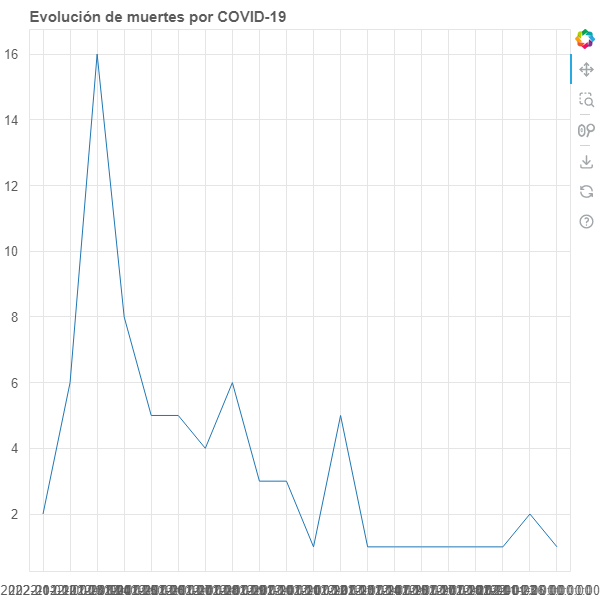
\includegraphics[width=\textwidth]{bokeh_linea}
		\caption{Implementación en Bokeh}
		\label{Fig: BokehLinea}
	\end{subfigure}
	\begin{subfigure}[b]{0.4\textwidth}
		\centering
		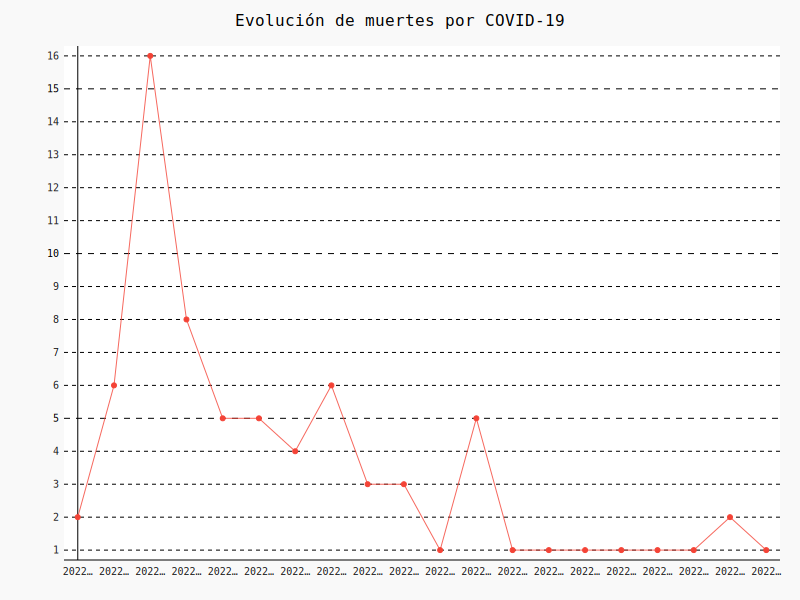
\includegraphics[width=\textwidth]{pygal_linea}
		\caption{Implementación en Pygal}
		\label{Fig: PygalLinea}
	\end{subfigure}
	\caption{Implementación de gráfico de línea en diversos paquetes de visualización de datos.}
	\label{Fig: Linea}
\end{figure}

\subsubsection{Gráfico de barras}
La Figra \ref{Fig: Barras} muestra el resultado de la implementación de un gráfico de barras en los paquetes de visualización de datos \emph{Bokeh} (Figura \ref{Fig: BokehBarras}) y \emph{Pygal} (Figura \ref{Fig: PygalBarras}).

\begin{figure}[!htb]
	\centering
	\begin{subfigure}[b]{0.4\textwidth}
		\centering
		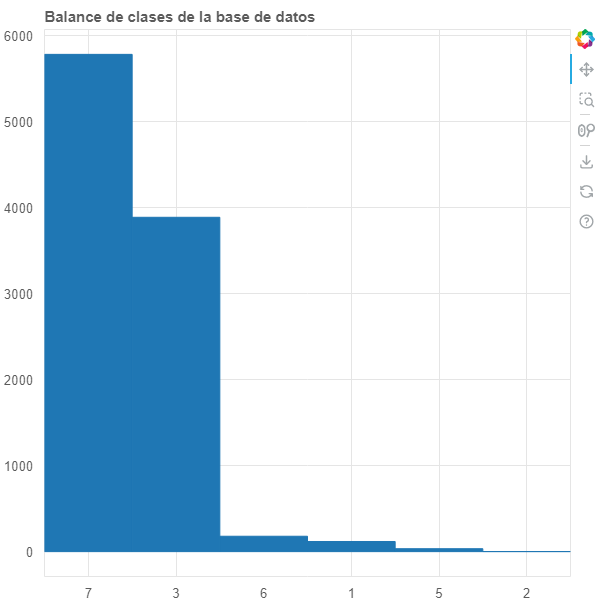
\includegraphics[width=\textwidth]{bokeh_barras}
		\caption{Implementación en Bokeh}
		\label{Fig: BokehBarras}
	\end{subfigure}
	\begin{subfigure}[b]{0.4\textwidth}
		\centering
		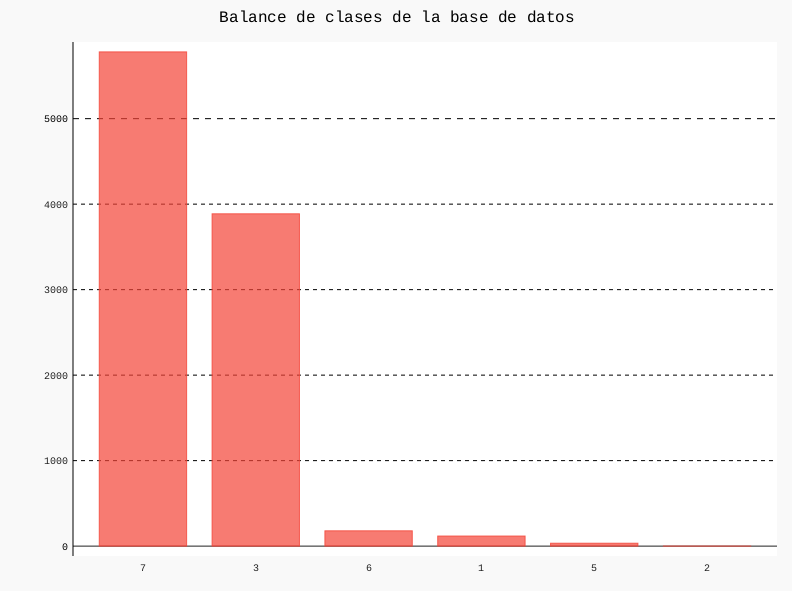
\includegraphics[width=\textwidth]{pygal_barras}
		\caption{Implementación en Pygal}
		\label{Fig: PygalBarras}
	\end{subfigure}
	\caption{Implementación de gráfico de barras en diversos paquetes de visualización de datos.}
	\label{Fig: Barras}
\end{figure}

\newpage

\subsubsection{Histograma}
La Figra \ref{Fig: Histograma} muestra el resultado de la implementación de un histograma en los paquetes de visualización de datos \emph{Bokeh} (Figura \ref{Fig: BokehHistograma}) y \emph{Pygal} (Figura \ref{Fig: PygalHistograma}).

\begin{figure}[!htb]
	\centering
	\begin{subfigure}[b]{0.4\textwidth}
		\centering
		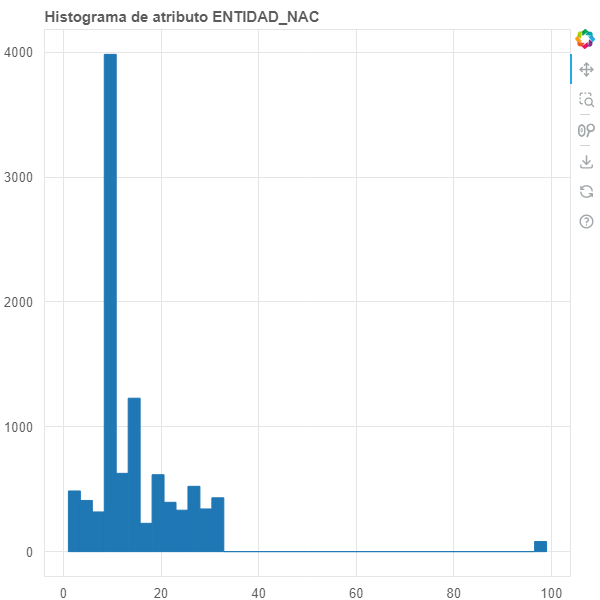
\includegraphics[width=\textwidth]{bokeh_histograma}
		\caption{Implementación en Bokeh}
		\label{Fig: BokehHistograma}
	\end{subfigure}
	\begin{subfigure}[b]{0.4\textwidth}
		\centering
		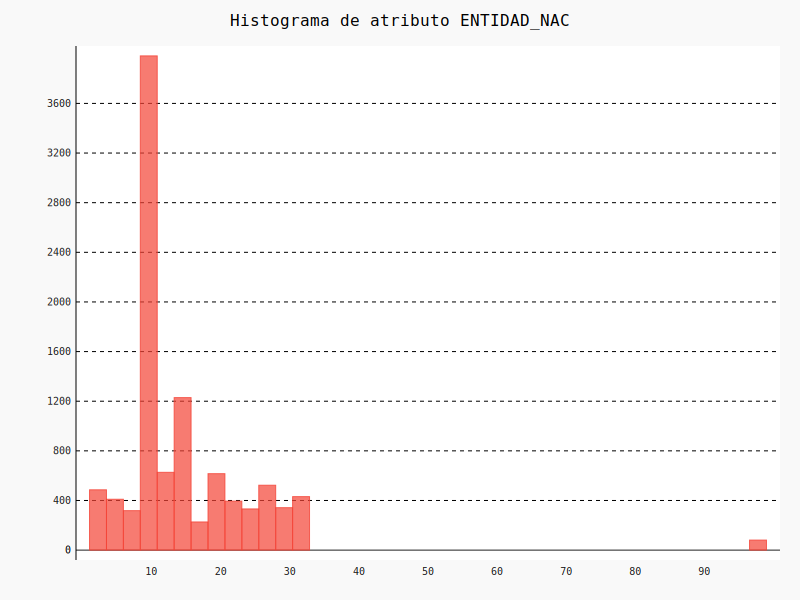
\includegraphics[width=\textwidth]{pygal_histograma}
		\caption{Implementación en Pygal}
		\label{Fig: PygalHistograma}
	\end{subfigure}
	\caption{Implementación de histograma en diversos paquetes de visualización de datos.}
	\label{Fig: Histograma}
\end{figure}

\subsubsection{Gráfico de dispersión}
La Figra \ref{Fig: Dispersion} muestra el resultado de la implementación de un gráfico de dispersión en los paquetes de visualización de datos \emph{Bokeh} (Figura \ref{Fig: BokehDispersion}) y \emph{Pygal} (Figura \ref{Fig: PygalDispersion}).

\begin{figure}[!htb]
	\centering
	\begin{subfigure}[b]{0.4\textwidth}
		\centering
		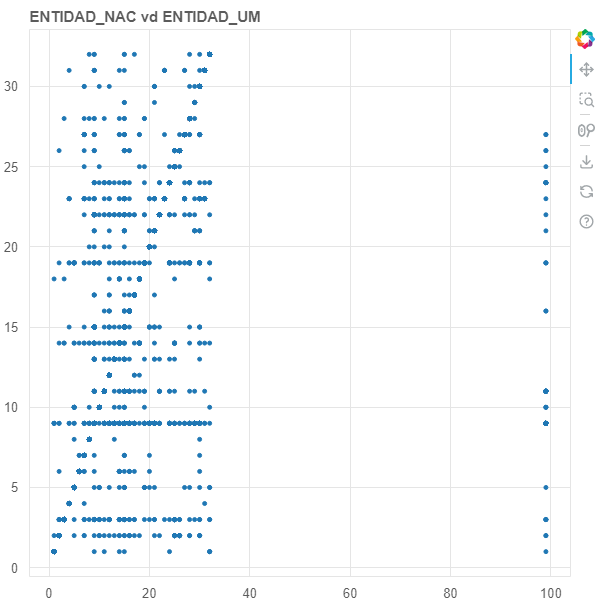
\includegraphics[width=\textwidth]{bokeh_dispersion}
		\caption{Implementación en Bokeh}
		\label{Fig: BokehDispersion}
	\end{subfigure}
	\begin{subfigure}[b]{0.4\textwidth}
		\centering
		\includegraphics[width=\textwidth]{pygal_dispersion}
		\caption{Implementación en Pygal}
		\label{Fig: PygalDispersion}
	\end{subfigure}
	\caption{Implementación de gráfico de dispersión en diversos paquetes de visualización de datos.}
	\label{Fig: Dispersion}
\end{figure}

\subsubsection{Gráfico de pastel}
La Figra \ref{Fig: Pastel} muestra el resultado de la implementación de un gráfico de pastel en los paquetes de visualización de datos \emph{Bokeh} (Figura \ref{Fig: BokehPastel}) y \emph{Pygal} (Figura \ref{Fig: PygalPastel}).

\begin{figure}[!htb]
	\centering
	\begin{subfigure}[b]{0.4\textwidth}
		\centering
		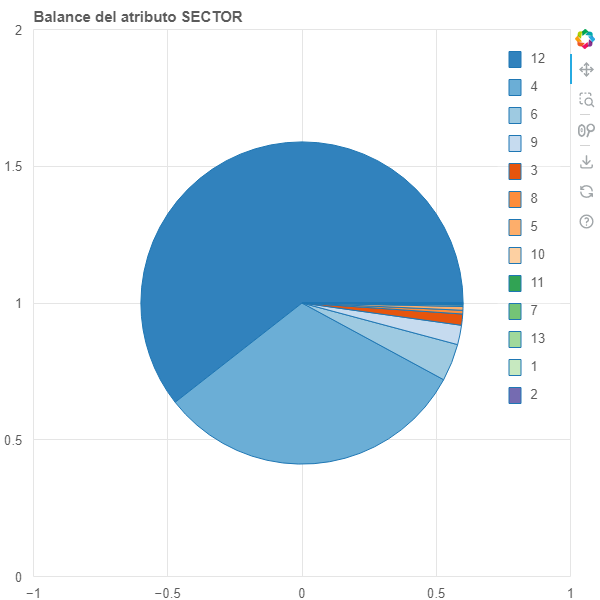
\includegraphics[width=\textwidth]{bokeh_pastel}
		\caption{Implementación en Bokeh}
		\label{Fig: BokehPastel}
	\end{subfigure}
	\begin{subfigure}[b]{0.4\textwidth}
		\centering
		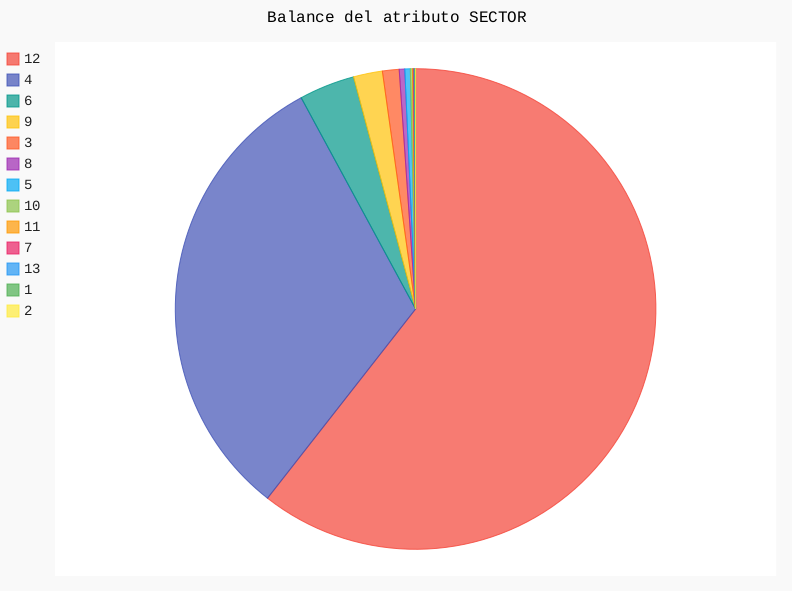
\includegraphics[width=\textwidth]{pygal_pastel}
		\caption{Implementación en Pygal}
		\label{Fig: PygalPastel}
	\end{subfigure}
	\caption{Implementación de gráfico de pastel en diversos paquetes de visualización de datos.}
	\label{Fig: Pastel}
\end{figure}

\newpage

\subsubsection{Diagrama de cajas}
La Figra \ref{Fig: Cajas} muestra el resultado de la implementación de un diagrama de cajas en los paquetes de visualización de datos \emph{Bokeh} (Figura \ref{Fig: BokehCajas}) y \emph{Pygal} (Figura \ref{Fig: PygalCajas}).

\begin{figure}[!htb]
	\centering
	\begin{subfigure}[b]{0.4\textwidth}
		\centering
		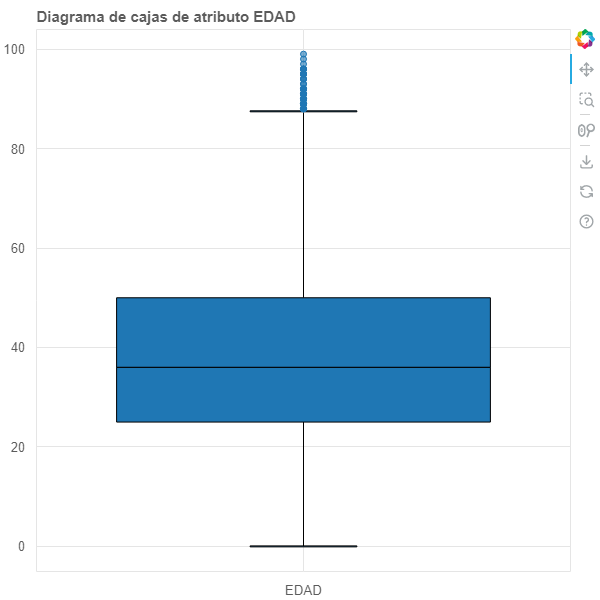
\includegraphics[width=\textwidth]{bokeh_cajas}
		\caption{Implementación en Bokeh}
		\label{Fig: BokehCajas}
	\end{subfigure}
	\begin{subfigure}[b]{0.4\textwidth}
		\centering
		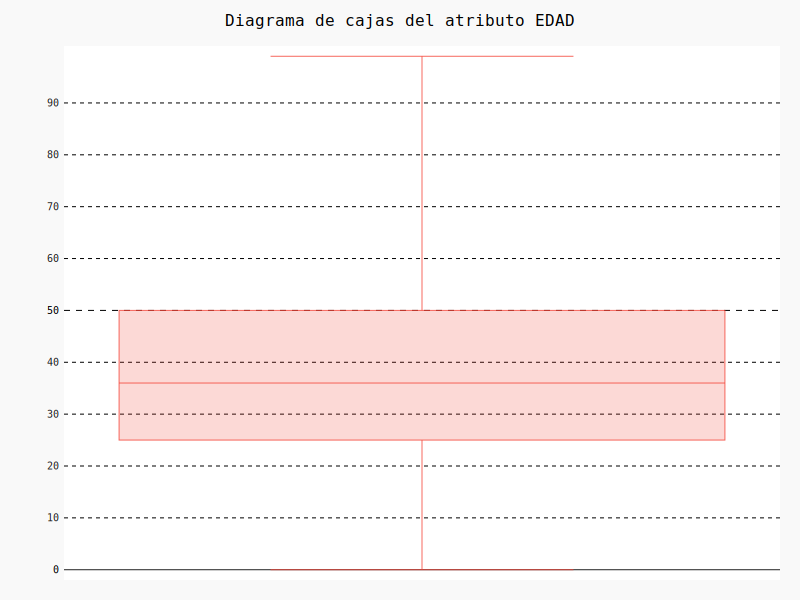
\includegraphics[width=\textwidth]{pygal_cajas}
		\caption{Implementación en Pygal}
		\label{Fig: PygalCajas}
	\end{subfigure}
	\caption{Implementación de diagrama de cajas en diversos paquetes de visualización de datos.}
	\label{Fig: Cajas}
\end{figure}

